\documentclass{standalone}

\usepackage{ifthen}
\usepackage{tikz}
\usetikzlibrary{arrows.meta}

\begin{document}

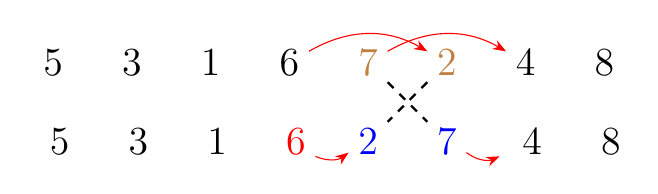
\begin{tikzpicture}[swap/.style = {dashed, thick},
	inv/.style = {>=Stealth, ->, red},
	ele/.style = {font = \Large}]
  \foreach \e [count = \ei] in {5,3,1,6,7,2,4,8} {
	  \node (2\e) [ele] at (\ei, 2) {\ifthenelse{\e = 7 \OR \e = 2}{\textcolor{brown}{$\e$}}{$\e$}};
  }

  \foreach \e [count = \ei] in {5,3,1,6,2,7,4,8} {
	  \node (1\e) [ele] at (\ei, 1) {\ifthenelse{\e = 7 \OR \e = 2}{\textcolor{blue}{$\e$}}{
		  \ifthenelse{\e = 6}{\textcolor{red}{$\e$}}{$\e$}}};
  }

  \draw [swap] (27) to (17);
  \draw [swap] (22) to (12);

  \draw [inv, bend left] (26) to (22);
  \draw [inv, bend left] (27) to (24);
  \draw [inv, bend right] (16) to (12);
  \draw [inv, bend right] (17) to (14);
\end{tikzpicture}
\end{document}